%% Securing the Game Build: A Sector Profile of SSDF and SLSA and a Self-Assessment Model for Independent Studios
%% Author: Osita Sean Keluo-Udeke
%% Prepared for: ACM Digital Threats: Research and Practice (DTRAP)
%% Part of the Open Build and Agent Assurance Framework (OBAAF).
%%
%% Build with pdfLaTeX + BibTeX. On Overleaf: New Project > Upload Project > the zip.
%% Requires the acmart class (part of TeX Live; preinstalled on Overleaf).
%%
%% Other venues:
%%   ACM Games: Research and Practice (alternative journal): replace \acmJournal{DTRAP}
%%   with \acmJournal{GAMES}. If your acmart version does not know GAMES, change acmsmall
%%   to manuscript in the class line and delete the \acmJournal line.
%% For double-anonymous review, add the "anonymous" class option.
\documentclass[acmsmall,screen,review]{acmart}

\acmJournal{DTRAP}
%% Submission copy: no ACM rights block or reference format yet.
\setcopyright{none}
\settopmatter{printacmref=false}
\renewcommand\footnotetextcopyrightpermission[1]{}

\usepackage{tabularx}
\usepackage{xltabular}
\usepackage{pdflscape}
\providecommand{\code}[1]{\texttt{#1}}
%% Large meet operator (n-ary greatest lower bound); defined only if the fonts lack one.
\providecommand{\bigsqcap}{\mathop{\vcenter{\hbox{\Large$\sqcap$}}}}
%% Let TeX stretch spaces a little more before overfilling a line.
\setlength{\emergencystretch}{1.5em}

\begin{document}

\title[Securing the Game Build]{Securing the Game Build: A Sector Profile of SSDF and SLSA and a Self-Assessment Model for Independent Studios}

\author{Osita Sean Keluo-Udeke}
\affiliation{%
  \institution{Affiliation to be confirmed}
  \city{Austin}
  \state{Texas}
  \country{USA}}
\email{seankudeke@gmail.com}

\renewcommand{\shortauthors}{Keluo-Udeke}

\begin{abstract}
Video games reach a majority of Americans through frequent updates, and attackers have repeatedly compromised game build, signing, and distribution systems to deliver malware through those updates. The leading guidance on build integrity (NIST's Secure Software Development Framework, NIST SP 800-204D, and SLSA) is sector-neutral. It assumes source-dominated repositories, dependencies delivered through package registries, builds that can run in fresh containers, and a release channel the producer controls. Game development departs from each assumption.

This paper develops the build-assurance component of the Open Build and Agent Assurance Framework (OBAAF), an open framework for securing build pipelines and the AI agents that operate in them, for its first target sector: video games. We review nine documented compromises of game build, signing, and distribution paths from 2013 to 2025 and identify seven properties of game development that break assumptions in generic guidance. We then construct a \emph{game-pipeline integrity profile} of 28 requirements that tailors the SSDF and SLSA to game builds, with a tiered isolation model for build hosts that cannot meet SLSA Build Level 3, controls for shared derived-data caches, and provenance verified before platforms take over distribution. For studios without security staff, we design a self-assessment of 34 observable yes-or-no items in four cumulative tiers.

An analytical evaluation maps every documented compromise to profile controls and assessment items, and every SLSA Build-track requirement to at least one item. We close with a protocol for piloting the assessment with independent U.S. studios. A companion paper supplies OBAAF's controls for AI agents.
\end{abstract}

%% CCS concepts: confirm or regenerate at https://dl.acm.org/ccs before submission.
\ccsdesc[500]{Security and privacy~Software security engineering}
\ccsdesc[300]{Security and privacy~Domain-specific security and privacy architectures}
\ccsdesc[100]{Applied computing~Computer games}

\keywords{software supply chain security, video games, build integrity, SSDF, SLSA, maturity models, small organizations}

\maketitle

\section{Introduction}\label{sec:1}

In 2025, 205.1 million Americans played video games for at least an hour a week~\cite{entertainment2025annual}. They receive those games, and a steady stream of updates to them, from an industry with 8,998 sites across all 50 states~\cite{grueber2026video}. Every update is produced by a build pipeline and signed or published under the studio's name, which makes the pipeline a route to the devices of everyone who trusts the game.

Attackers have used that route for more than a decade. A campaign reported in 2013 compromised at least 35 game companies, stole more than a dozen code-signing certificates, and delivered a trojan through a publisher's official update server~\cite{kaspersky2013winnti}. A state-linked group reported in 2019 reached game production environments, stole source code and certificates, and injected malicious code into legitimate files that were later distributed~\cite{mandiant2019apt41}. The same year, researchers found that attackers had altered the build configuration of two games and a gaming platform application, so that the official executables carried a backdoor~\cite{eset2019gaming}; in 2020 the group reached a game developer's build orchestration server~\cite{eset2020winnti}. More recently, attackers used compromised developer accounts to push malicious updates to released games on Steam, prompting Valve to require SMS confirmation before builds go live~\cite{toulas2023steam}, and hijacked a mod developer's account to ship an infostealer as an update~\cite{gatlan2023steam}.

The leading guidance on build integrity does not speak to this sector directly. NIST's Secure Software Development Framework (SSDF)~\cite{souppaya2022secure,booth2025secure}, its guidance on CI/CD pipelines in SP 800-204D~\cite{chandramouli2024strategies}, and the SLSA framework~\cite{openndslsa} are deliberately sector-neutral. They assume, without saying so, that source code dominates a repository, that dependencies arrive through package registries with metadata, that a build can run in a fresh container, and that the producer's own signature reaches the user. Game pipelines violate each assumption. NIST's answer to sector-specific needs is the \emph{community profile}, which tailors a general framework to a shared context. It has published such a profile of the SSDF for AI model development~\cite{booth2024secure} and a guide to creating community profiles of its Cybersecurity Framework~\cite{pascoe2024nist}. No such profile exists for game development.

The gap matters most for the studios least able to fill it themselves. Of the 1,767 U.S. video game software sites identified in a 2026 economic study, 1,276 have between one and nine employees~\cite{grueber2026video}. In a 2025 survey of more than 3,000 developers, 59\% worked at companies of 50 people or fewer~\cite{game2025state}. Outcome-based frameworks leave studios of that size to work out on their own what each practice means for an engine, a set of console toolchains, and a storefront account.

This paper develops the build-assurance component of the Open Build and Agent Assurance Framework (OBAAF) for video game studios and makes four contributions:

\begin{enumerate}
\item A review of nine documented compromises of game build, signing, and distribution paths (\S\ref{sec:3}), which identifies the attack paths they share.
\item Seven properties of game development that break assumptions in generic guidance (\S\ref{sec:4}), each grounded in engine documentation, platform requirements, or empirical studies.
\item A game-pipeline integrity profile (\S\ref{sec:5}) of 28 requirements in nine control families, tailoring the SSDF and SLSA to game builds.
\item A four-tier self-assessment of 34 yes-or-no items for studios without security staff (\S\ref{sec:6}), designed with an established procedure for developing maturity models, with an analytical evaluation (\S\ref{sec:7}) and a pilot protocol (\S\ref{sec:8}).
\end{enumerate}

This paper is the second of two that together define OBAAF. The companion paper develops the framework's agent-assurance component, a set of controls for AI agents that operate inside build pipelines~\cite{keluoudeke2026untrusted}; here we adopt its pipeline model and incorporate its requirements as one control family.


\section{Background}\label{sec:2}


\subsection{Build-integrity frameworks and community profiles}\label{sec:2.1}

The SSDF organizes secure development into four groups of practices: preparing the organization (PO), protecting the software (PS), producing well-secured software (PW), and responding to vulnerabilities (RV)~\cite{souppaya2022secure}. Its draft version 1.2 adds a practice on making software updates robust and reliable (PS.4)~\cite{booth2025secure}. The practices are deliberately outcome-based: they say what to achieve, not how to achieve it in a particular toolchain.

SLSA expresses build integrity as levels on two tracks~\cite{openndslsa}. On the Build track, Level 1 requires provenance describing how an artifact was built, Level 2 requires that provenance to be signed and generated by a hosted build platform, and Level 3 requires a hardened platform. At Level 3, an ephemeral build environment must be provisioned for each build, overlapping builds must not influence one another, caches must not be a route for poisoning, and signing material must be inaccessible to user-defined build steps. On the Source track, levels rise from version control to change history and provenance, continuous technical controls on protected branches, and two-party review. in-toto supplies the attestation format that ties the steps of a pipeline together~\cite{torresarias2019toto}, and Sigstore makes signing practical by binding short-lived certificates to workload identities~\cite{newman2022sigstore}. Reproducible builds offer independent verification that a binary came from its claimed source~\cite{lamb2022reproducible}, though practitioners describe them as important but laborious~\cite{fourne2023it}.

A \emph{community profile} adapts a general framework to a shared context. NIST's SSDF profile for generative AI adds practices, tasks, and notes specific to AI model development~\cite{booth2024secure}, and NIST's guide to community profiles of its Cybersecurity Framework describes them as capturing shared interests, goals, and outcomes for a sector, technology, or challenge~\cite{pascoe2024nist}. We follow this model: our profile adds tailoring and notes to the SSDF and SLSA rather than replacing them.


\subsection{How games are built}\label{sec:2.2}

A game's repository is dominated by content rather than code. In a study of open-source projects, multimedia assets made up as much as 70\% of some game repositories but less than 5\% of non-game ones, and development files were about 30\% of game repositories against about 80\% elsewhere~\cite{pascarella2018how}. Studies of commercial development describe a discipline with creative, multidisciplinary requirements~\cite{murphyhill2014cowboys}, and an analysis of 200 postmortems found that the industry's problems are mainly people-related~\cite{politowski2021game}.

A typical pipeline runs in four stages.

\begin{enumerate}
\item \emph{Author and import.} Artists and designers create assets in content tools and import them into an engine. Engines run editor code during this stage: Unity, for example, runs scripts marked with its \code{InitializeOnLoad} attribute whenever the editor launches or recompiles scripts~\cite{unityndrunning}.
\item \emph{Cook and cache.} The engine converts assets into platform formats. Unreal Engine stores the results in a derived-data cache that a team and its build machines can share, so that ``only one person at any given time needs to build the derived data'' for an asset~\cite{epicndusing}. Engine documentation also warns that cooking can be intermittently nondeterministic~\cite{epicndc}.
\item \emph{Compile, package, and sign per platform.} The same project is built for several platforms, each with its own toolchain and signing rules. Apple platforms require executable code signed with an Apple-issued certificate~\cite{applendapp}. On Google Play, Google holds the app-signing key and the studio signs uploads with a separate upload key~\cite{googlenduse}.
\item \emph{Publish and update.} Builds are uploaded to storefronts or to the studio's own launcher. Steam recommends a dedicated build account for uploads and requires a person, rather than an automated step, to set a build live on a released game's default branch~\cite{valvenduploading}. Console toolchains are available only under contract to approved developers~\cite{godotndconsole}.
\end{enumerate}

Updates are frequent. Among popular Steam games, those that follow a frequent-update strategy release a higher share of same-day updates~\cite{lin2017studying}, and 16\% of developers in a 2025 survey were working on live-service games~\cite{game2025state}.


\subsection{Pipeline model and terms}\label{sec:2.3}

We adopt OBAAF's pipeline model, defined in the companion paper~\cite{keluoudeke2026untrusted}. A pipeline has a \emph{source plane} (repositories and protected branches), a \emph{trigger plane} (events that start workflows), an \emph{execution plane} (build hosts), a \emph{credential plane} (tokens and keys), and a \emph{release plane} (signing, publication, and provenance). Principals are ordered by trust as Public, Contributor, Maintainer, and Release. Work is separated into \emph{lanes}: untrusted work runs in a lane without secrets, and release builds run in a separate lane that never processes unreviewed changes. The companion paper's requirements for AI agents (R1–R8) appear here as control family F8.


\section{Documented compromises of game build and distribution paths}\label{sec:3}


\subsection{Method}\label{sec:3.1}

We searched threat-intelligence reports, platform notices, and security journalism for incidents from 2013 to 2025 in which a game's build environment, signing material, third-party components, or publishing and update channel was compromised and used, or positioned, to deliver malicious code to players. We read each primary source and included cases with a documented compromise and a described path to players. Breaches that exposed source code without affecting what players received fall outside our scope. Nine cases met the criteria (Table~\ref{tab:1}). For two of them, the public record does not establish whether a legitimate developer was compromised or the publisher itself was malicious; we include them because both reached players as updates to titles already on a major store, and we mark their attack path as presumed.

We coded each case by attack path:

\begin{itemize}
\item \emph{AP1, build environment:} the attacker altered what the studio's own build produced.
\item \emph{AP2, signing material:} the attacker stole certificates or keys and signed malware as the studio.
\item \emph{AP3, publishing or update channel:} the attacker pushed a malicious update through an account, server, or store the players trusted.
\item \emph{AP4, third-party component:} malicious code arrived inside an SDK or dependency the studio shipped.
\end{itemize}

\begin{table}[htbp]
\caption{Documented compromises of game build, signing, and distribution paths.}
\label{tab:1}
\footnotesize
\begin{tabularx}{\linewidth}{@{}>{\hsize=0.974\hsize\raggedright\arraybackslash}X>{\hsize=1.293\hsize\raggedright\arraybackslash}X>{\hsize=1.293\hsize\raggedright\arraybackslash}X>{\hsize=0.684\hsize\raggedright\arraybackslash}X>{\hsize=0.756\hsize\raggedright\arraybackslash}X@{}}
\toprule
\textbf{Case (reported)} & \textbf{What was compromised} & \textbf{Path to players} & \textbf{Status} & \textbf{Attack path} \\
\midrule
Winnti campaign \cite{kaspersky2013winnti} (2013) & At least 35 game companies; source code and more than a dozen code-signing certificates & A trojan delivered through a publisher's official update server; stolen certificates used to sign malware & Exploited & AP2, AP3 \\
APT41 \cite{mandiant2019apt41} (2019) & Game production environments, source code, and certificates & Malicious code injected into legitimate files that were later distributed; malware signed with stolen certificates & Exploited & AP1, AP2 \\
Winnti build compromises \cite{eset2019gaming} (2019) & Build configuration of two games and one gaming platform application, which hooked C runtime initialization & Backdoored official executables, with victims estimated in the tens or hundreds of thousands & Exploited & AP1 \\
PipeMon \cite{eset2020winnti} (2020) & Build orchestration server at massively multiplayer game developers; backdoor signed with a previously stolen certificate & Could have trojanized game executables; no evidence that it did & Access gained & AP1, AP2 \\
SpinOk \cite{doctor2023android} (2023) & A marketing SDK embedded in apps and games & A spyware module in 101 apps with more than 421 million downloads & Exploited & AP4 \\
Steamworks accounts \cite{toulas2023steam} (2023) & Developer publishing accounts & Malicious updates pushed to released games; Valve notified a few hundred affected users & Exploited & AP3 \\
Downfall mod \cite{gatlan2023steam} (2023) & A developer's Steam and Discord accounts, likely through session-token theft & A malicious update, live for about an hour, that installed an infostealer & Exploited & AP3 \\
Chemia \cite{mott2025hacker} (2025) & An early-access Steam game; origin of the change undetermined & Updates carrying three malware families & Exploited & AP3 (presumed) \\
BlockBlasters \cite{toulas2025verified,tan2025infected} (2025) & A verified free Steam game; origin of the change undetermined & A patch released a month after launch that delivered a cryptocurrency stealer, with reported losses of about \$150,000 & Exploited & AP3 (presumed) \\
\bottomrule
\end{tabularx}
\end{table}

Several techniques documented outside the game industry apply directly to game pipelines (Table~\ref{tab:2}). We use them in \S\ref{sec:7} to test the profile against attacks that have not yet been reported in games.

\begin{table}[htbp]
\caption{Techniques from other sectors that transfer to game pipelines.}
\label{tab:2}
\small
\begin{tabularx}{\linewidth}{@{}>{\hsize=0.566\hsize\raggedright\arraybackslash}X>{\hsize=1.288\hsize\raggedright\arraybackslash}X>{\hsize=1.147\hsize\raggedright\arraybackslash}X@{}}
\toprule
\textbf{Case} & \textbf{Technique} & \textbf{Relevance to games} \\
\midrule
SUNSPOT \cite{crowdstrike2021sunspot} (2021) & Malware on the build server swapped a source file during compilation and restored it afterward, so the repository stayed clean & Source review alone cannot detect build-time tampering \\
3CX \cite{mandiant20233cx} (2023) & Attackers compromised Windows and macOS build environments and shipped trojanized, signed installers & Multi-platform build fleets multiply the hosts to defend \\
PyTorch \cite{stawinski2024playing} (2024) & Persistent self-hosted runners ran workflows from pull requests and exposed release credentials & Persistent build hosts are common where toolchains resist containers \\
Ultralytics \cite{larson2024supply} (2024) & A poisoned CI cache was consumed by the release build & Engines share derived-data caches across teams and build machines \\
tj-actions \cite{stepsecurity2025harden} (2025) & A widely used CI component was altered to dump secrets into build logs & Pipelines run third-party components with release credentials in reach \\
Clinejection \cite{khan2026clinejection} (2026) & An AI triage workflow, steered by an issue title, poisoned a cache used by release jobs and exposed publishing tokens & Studios adopting AI agents in pipelines inherit the same risk \\
\bottomrule
\end{tabularx}
\end{table}


\subsection{Findings}\label{sec:3.2}

\emph{Every path ends at a channel players already trust.} Players received malicious code through official executables, signed binaries, an official update server, and store updates. None required players to do anything unusual.

\emph{Signing material and publishing accounts are as valuable as source code.} Three cases involved stolen code-signing certificates~\cite{kaspersky2013winnti,mandiant2019apt41,eset2020winnti}, and at least three cases used publishing accounts or update infrastructure~\cite{kaspersky2013winnti,toulas2023steam,gatlan2023steam}. Controls that protect only the repository miss both.

\emph{Build-time tampering leaves the source clean.} In the 2019 compromises, attackers changed the build configuration rather than the source~\cite{eset2019gaming}, as SUNSPOT later did through a file swap during compilation~\cite{crowdstrike2021sunspot}. Detection therefore requires evidence about the build itself: provenance, host integrity, or an independent rebuild.

\emph{Platforms are adding controls on their side.} Valve's SMS confirmation~\cite{toulas2023steam} and its rule that a person must set a released game's default branch live~\cite{valvenduploading} are platform-side versions of the release gates we propose. A studio's pipeline must meet them halfway, since a platform cannot tell a legitimate update from one built by an attacker with the studio's credentials.

These paths fit within existing taxonomies of software supply chain attacks~\cite{ladisa2023sok} and their defensive properties of transparency, validity, and separation~\cite{okafor2022sok}. What differs in games is where each path runs, which the next section examines.


\section{Where generic guidance meets game pipelines}\label{sec:4}

Seven properties of game development break assumptions that generic build-integrity guidance makes without stating them. Table~\ref{tab:3} lists each property, the evidence for it, the assumption it breaks, and how the profile in \S\ref{sec:5} responds.

\begingroup
\footnotesize
\begin{xltabular}{\linewidth}{@{}>{\hsize=0.849\hsize\raggedright\arraybackslash}X>{\hsize=1.050\hsize\raggedright\arraybackslash}X>{\hsize=1.050\hsize\raggedright\arraybackslash}X>{\hsize=1.050\hsize\raggedright\arraybackslash}X@{}}
\caption{Properties of game development that break assumptions in generic guidance.}\label{tab:3}\\
\toprule
\textbf{Property} & \textbf{Evidence} & \textbf{Assumption broken} & \textbf{Profile response} \\
\midrule
\endfirsthead
\multicolumn{4}{@{}l}{\emph{Table~\ref{tab:3}, continued}}\\
\toprule
\textbf{Property} & \textbf{Evidence} & \textbf{Assumption broken} & \textbf{Profile response} \\
\midrule
\endhead
\bottomrule
\endlastfoot
D1. Assets dominate inputs, and some can execute code & Assets make up as much as 70\% of some game repositories \cite{pascarella2018how}; Unity runs marked editor code whenever the editor launches or recompiles \cite{unityndrunning}; 3D model files have carried scripts that run when the file is opened with automatic script execution enabled \cite{uzan2025morphisec}; engine resource packs have carried executable scripts \cite{gatlan2024hackers} & The material entering a build is source code that people review & Treat third-party assets and plugins as code at intake (F2) \\
D2. Engines, middleware, and platform SDKs arrive outside package registries & Console SDKs and export templates are shared privately with approved developers under contract \cite{godotndconsole}; a marketing SDK embedded in games carried a spyware module \cite{doctor2023android} & Dependencies arrive through registries with metadata that tools can read & A binary manifest with digests, and review of player-facing SDKs (F2) \\
D3. One project fans out to platform-specific build hosts, some persistent & Apple platforms require Apple-issued signing \cite{applendapp}; some platforms need their own operating system to build, so container images cannot cover them \cite{gamecinddocker}; hosted runners can supply a fresh virtual machine per job \cite{githubndgithub}, but console toolchains are available only under contract \cite{godotndconsole}; attackers have compromised Windows and macOS build environments \cite{mandiant20233cx} and persistent runners \cite{stawinski2024playing} & Every build can run in a fresh, isolated environment, as SLSA Build Level 3 requires \cite{openndslsa} & Tiered isolation with compensating controls for persistent hosts (F3) \\
D4. Builds depend on shared, writable derived-data caches & Unreal's shared cache makes derived data built by one person available to all users and build machines \cite{epicndusing}; engine documentation warns that cooking can be intermittently nondeterministic \cite{epicndc}; cache poisoning has reached release builds elsewhere \cite{larson2024supply,khan2026clinejection} & Builds are hermetic and reproducible, so caches are only an optimization & Lane-scoped caches and verified derived data for releases (F4) \\
D5. Platforms take over signing and distribution & Google signs the distributed app with a key it holds \cite{googlenduse}; Apple requires Apple-issued certificates \cite{applendapp}; Steam requires a dedicated build account and a person to set a released build live \cite{valvenduploading}, and SMS confirmation since 2023 \cite{toulas2023steam} & The producer's signature reaches the user, who can verify the producer's provenance & Verify provenance before upload, and protect upload credentials as release keys (F6, F7) \\
D6. Updates are frequent and often urgent & Frequently updated Steam games release a higher share of same-day updates \cite{lin2017studying}; 16\% of surveyed developers work on live-service games \cite{game2025state}; SSDF 1.2 adds a practice on robust updates \cite{booth2025secure} & Releases are infrequent enough for heavyweight manual review & Automated provenance gates that hotfixes cannot skip, plus staged rollout (F6, F7) \\
D7. Most studios are small and rely on partners & 1,276 of 1,767 U.S. game software sites have one to nine employees \cite{grueber2026video}; 59\% of surveyed developers work at companies of 50 or fewer \cite{game2025state}; console ports often go through third-party vendors \cite{godotndconsole}; the industry's problems are mainly people-related \cite{politowski2021game} & An organization can staff a security program to interpret outcome-based practices & Plain-language, tiered self-assessment (\S\ref{sec:6}) and scoped partner access (F9) \\
\end{xltabular}
\endgroup

Two consequences follow. First, the boundary of ``source'' must widen. In a game, an asset package, an editor plugin, or a vendor's platform library can change what ships as surely as a code commit, yet none passes through the review and dependency tooling that generic guidance assumes. Second, the boundary of ``release'' must move earlier. Because platforms re-sign, gate, and distribute builds (D5), the last point at which a studio can bind an artifact to its own pipeline is the moment before upload. Provenance that is not checked there cannot be checked by anyone downstream.

D7 shapes everything else. Guidance for small organizations has long favored fundamentals stated in non-technical language~\cite{paulsen2016small}, and surveys of small and medium businesses report limited security resources and expertise~\cite{chidukwani2022survey}. A profile that requires interpretation by specialists will not be adopted by most of the studios it is meant to protect, which is why \S\ref{sec:6} pairs the profile with a self-assessment.


\section{The game-pipeline integrity profile}\label{sec:5}


\subsection{Structure}\label{sec:5.1}

The profile has 28 requirements in nine control families, each guarding one step on the path from studio to player (Figure~\ref{fig:1}). Every requirement names the attack paths of \S\ref{sec:3} and the properties of \S\ref{sec:4} it addresses, and maps to SSDF practices and, where one applies, a SLSA requirement or another framework. Following NIST's practice for community profiles~\cite{booth2024secure,pascoe2024nist}, the profile tailors and annotates existing practices rather than defining new ones, except where \S\ref{sec:4} shows a gap.

\begin{figure}[htbp]
\centering
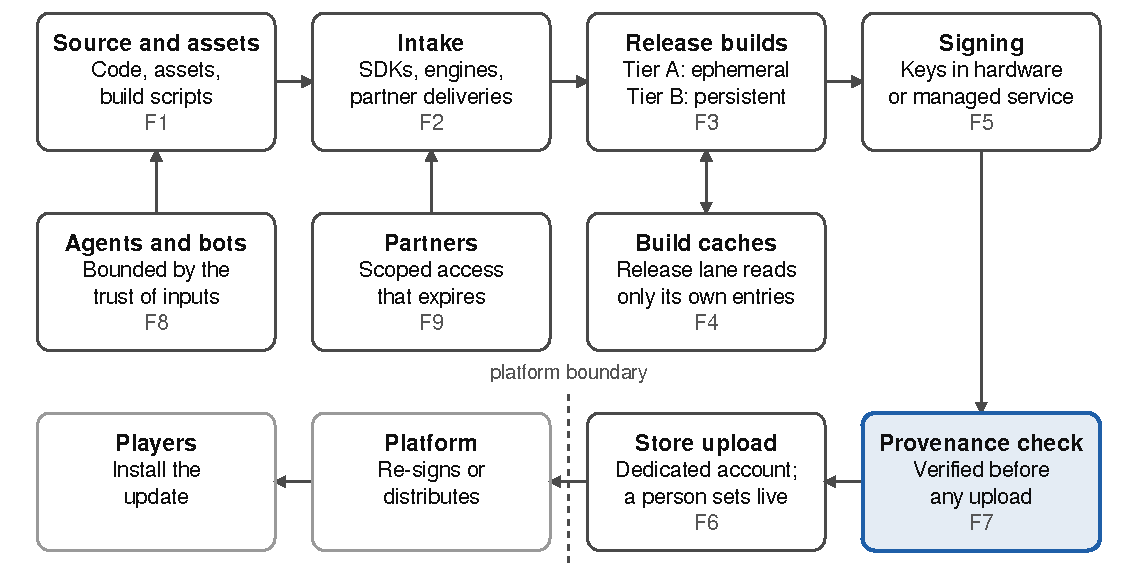
\includegraphics[width=\linewidth]{figures/fig1-control-families.pdf}
\caption{Control families F1–F9 along the path from studio to player. Everything left of the platform boundary in the lower row is outside the studio's control, which is why provenance is verified (F7) before upload rather than after.}
\Description{A diagram of the path from a game studio to players. The top row shows source and assets (F1), intake of SDKs and partner deliveries (F2), release builds in Tier A or Tier B (F3), and signing (F5). Below them sit agents and bots (F8), partners (F9), and build caches (F4). The bottom row runs from a provenance check (F7) to store upload (F6), then across a dashed platform boundary to the platform and finally the players.}
\label{fig:1}
\end{figure}

\begingroup
\footnotesize
\begin{xltabular}{\linewidth}{@{}>{\hsize=0.321\hsize\raggedright\arraybackslash}X>{\hsize=2.550\hsize\raggedright\arraybackslash}X>{\hsize=0.762\hsize\raggedright\arraybackslash}X>{\hsize=0.466\hsize\raggedright\arraybackslash}X>{\hsize=0.901\hsize\raggedright\arraybackslash}X@{}}
\caption{The game-pipeline integrity profile.}\label{tab:4}\\
\toprule
\textbf{ID} & \textbf{Requirement} & \textbf{Addresses} & \textbf{SSDF} & \textbf{SLSA or other} \\
\midrule
\endfirsthead
\multicolumn{5}{@{}l}{\emph{Table~\ref{tab:4}, continued}}\\
\toprule
\textbf{ID} & \textbf{Requirement} & \textbf{Addresses} & \textbf{SSDF} & \textbf{SLSA or other} \\
\midrule
\endhead
\bottomrule
\endlastfoot
\textbf{F1} & \textbf{Source and assets} &  &  &  \\
G1.1 & Protect release branches and streams: changes need review, and build scripts, CI configuration, and engine and plugin code are owner-protected paths & AP1 & PS.1 & Source L3 \\
G1.2 & Treat the build definition as code: build graphs and packaging and signing steps live in version control, changes need approval by someone other than the author, and build hosts take configuration only from version control & AP1; D3 & PS.1, PW.7 & Source L4, for the build definition \\
G1.3 & Attribute every change: individual accounts for every person and partner, with no shared logins & AP1; D7 & PS.1 & Source L2 \\
\textbf{F2} & \textbf{Intake of third-party code, SDKs, and assets} &  &  &  \\
G2.1 & Keep a binary manifest: record every vendored binary, SDK, engine build, and plugin with its source, version, and digest, and fail builds on unrecorded changes & AP4; D2 & PW.4, PS.3.2 & S2C2F ingest and inventory \cite{openndsecure} \\
G2.2 & Quarantine third-party assets and plugins: open them first in an isolated environment without credentials and with automatic script execution off, and review editor scripts before they enter the project & D1 & PW.4, PO.5 & - \\
G2.3 & Review each player-facing SDK for data access and network behavior before adoption and on each update & AP4; D2 & PW.4 & - \\
\textbf{F3} & \textbf{Build execution} &  &  &  \\
G3.1 & Separate the release lane: release builds run only on hosts that never build unreviewed changes and accept no interactive sessions & AP1; D3 & PO.5 & Build L3, isolation \\
G3.2 & Use tiered isolation: Tier A, a fresh environment per build where toolchains allow; Tier B, persistent hosts dedicated to the release lane, reimaged from a versioned image on a schedule and after any suspected exposure, with their builds reported as below Build L3 & AP1; D3 & PO.5 & Build L3, for Tier A \\
G3.3 & Restrict egress from release hosts to package mirrors, platform upload endpoints, and the provenance service & AP1 & PO.5 & - \\
G3.4 & Keep no standing secrets on build hosts: issue signing and upload credentials per job and short-lived, or use them through a signing service & AP2 & PO.5 & Build L3, unforgeable provenance \\
\textbf{F4} & \textbf{Derived data and caches} &  &  &  \\
G4.1 & Scope caches by lane: caches written by untrusted builds, workstations, or partners are never read by release builds & AP1; D4 & PO.5 & Build L3, cache integrity \\
G4.2 & Regenerate or verify derived data for releases: release builds rebuild derived data or consume only content-addressed entries written by the release lane & AP1; D4 & PS.1 & Build L3, cache integrity \\
G4.3 & Check code artifacts by independent rebuild, recording expected differences and known engine nondeterminism & AP1; D4 & PS.2 & Reproducible builds \cite{lamb2022reproducible} \\
\textbf{F5} & \textbf{Signing} &  &  &  \\
G5.1 & Hold signing and upload keys in hardware, a cloud key service, or platform-managed signing, and log every use & AP2; D5 & PS.2 & - \\
G5.2 & Sign only artifacts that carry valid release-lane provenance & AP1, AP2 & PS.2 & Build L2–L3 \\
G5.3 & Keep a written plan to revoke certificates and rotate upload credentials & AP2 & PS.2 & - \\
\textbf{F6} & \textbf{Distribution and updates} &  &  &  \\
G6.1 & Upload from a dedicated identity with only publishing permissions, as Steam recommends \cite{valvenduploading} & AP3; D5 & PO.5 & - \\
G6.2 & Require a person to set a build live on a public channel, and two people at the highest tier & AP3; D5 & PS.4 (draft 1.2) & Analogous to Source L4 \\
G6.3 & Protect every publishing account with multi-factor authentication, and alert on set-live events and permission changes & AP3 & PO.5 & - \\
G6.4 & Roll out live updates in stages, with a tested rollback & D6 & PS.4 (draft 1.2) & - \\
G6.5 & Make self-hosted launchers and patchers verify update signatures with keys not stored on the update server & AP3 & PS.2 & The Update Framework \cite{samuel2010survivable} \\
\textbf{F7} & \textbf{Provenance} &  &  &  \\
G7.1 & Emit signed provenance for every platform artifact, listing source revision, asset revision, manifest digest, SDK versions, and builder identity & AP1; D5 & PS.3.2 & Build L1–L2 \\
G7.2 & Verify provenance against policy, in a separate step, before any upload to a store & AP1, AP3; D5, D6 & PS.2 & Build-track verification \\
G7.3 & Archive released artifacts, symbols, and provenance read-only & All & PS.3.1 & - \\
\textbf{F8} & \textbf{Automation and AI agents} &  &  &  \\
G8.1 & Bound the authority of agents and bots by the trust of their inputs; agents triggered by player reports, community issues, or partner content run without secrets (companion R1–R4, R7) \cite{keluoudeke2026untrusted} & AP1, AP3 & PO.5 & - \\
G8.2 & Protect agent instruction and workflow files as code (companion R5) & AP1 & PS.1 & Source L3 \\
G8.3 & Attest agent runs, and verify agent-authored changes before release (companion R8) & AP1 & PS.3.2 & Build provenance \\
\textbf{F9} & \textbf{Partners} &  &  &  \\
G9.1 & Give contractors and porting partners separate, scoped, time-limited access, and build their contributions in the untrusted lane & AP1; D7 & PO.2, PO.5 & - \\
\end{xltabular}
\endgroup


\subsection{Key tailoring decisions}\label{sec:5.2}

\emph{Tiered isolation (G3.2).} SLSA Build Level 3 requires an ephemeral environment for every build~\cite{openndslsa}, and some platform builds cannot meet it with the infrastructure a studio has (D3). Rather than declare Level 3 impossible, or claim it where it is not met, the profile defines Tier B: persistent hosts that are dedicated to the release lane, never build unreviewed changes, accept no interactive sessions, restrict egress, hold no standing secrets, and are reimaged on a schedule. Tier B builds are reported as below Level 3 in their provenance. This keeps the SLSA claim truthful while closing the paths that compromised persistent hosts in the PyTorch and 3CX cases~\cite{mandiant20233cx,stawinski2024playing}.

\emph{Derived data as a build input (F4).} A shared derived-data cache is a productivity feature: data one person builds becomes available to every user and build machine~\cite{epicndusing}. If release builds read it, anyone who can write to it can influence what ships. The profile treats cache entries as build inputs with an author: release builds read only entries the release lane wrote, or regenerate them. Because cooking can be nondeterministic~\cite{epicndc}, independent rebuilds (G4.3) are required for code artifacts, where determinism is achievable, while cooked content relies on the provenance of cache entries.

\emph{Provenance at the platform boundary (G7.2).} When a platform re-signs a build, as Google Play does~\cite{googlenduse}, the studio's signature does not reach the player, and when a store distributes builds under account credentials, there may be no studio signature to check. Either way, the moment before upload is the last point at which a studio can bind an artifact to its pipeline. The profile places a mandatory verification step there and pairs it with the platform's own release gates~\cite{valvenduploading}.

\emph{Intake as a security boundary (F2).} Adapting the consumption practices of S2C2F~\cite{openndsecure} to games, the profile extends them from package registries to asset marketplaces, vendor portals, and partner deliveries, and treats any file that an editor or engine can execute as code.

\emph{Update channels the studio runs (G6.5).} The 2013 campaign distributed malware through an official update server~\cite{kaspersky2013winnti}. The Update Framework showed that update systems survive server compromise when signing keys are kept apart from the servers that distribute updates~\cite{samuel2010survivable}; the profile applies that principle to self-hosted launchers and patchers.

\emph{Agents in the pipeline (F8).} As studios add AI agents to triage player reports or repair builds, the controls of the companion paper apply~\cite{keluoudeke2026untrusted}. The Clinejection case shows why F4 and F8 must be read together: an agent influenced by an issue title reached release credentials through a shared cache~\cite{khan2026clinejection}.


\section{A self-assessment for studios without security staff}\label{sec:6}


\subsection{Design method}\label{sec:6.1}

We followed the procedure model of Becker et al. for developing maturity models~\cite{becker2009developing}. Its early phases are problem definition, comparison with existing models, iterative development, and a plan for transfer and evaluation. Section~\ref{sec:4} supplies the problem definition. This section reports the comparison and the first development iteration, and \S\ref{sec:8} specifies the evaluation.


\subsection{Comparison with existing models}\label{sec:6.2}

Existing models each cover part of the need (Table~\ref{tab:5}). None addresses assets, derived data, store accounts, or the platform boundary, and most assume an organization that can staff a security program.

\begin{table}[htbp]
\caption{Existing assessment models and their fit for small game studios.}
\label{tab:5}
\small
\begin{tabularx}{\linewidth}{@{}>{\hsize=0.428\hsize\raggedright\arraybackslash}X>{\hsize=1.286\hsize\raggedright\arraybackslash}X>{\hsize=1.286\hsize\raggedright\arraybackslash}X@{}}
\toprule
\textbf{Model} & \textbf{What it assesses} & \textbf{Gap for small game studios} \\
\midrule
OWASP SAMM \cite{owaspndsoftware} & 15 security practices in five business functions, each at three maturity levels; intended for organizations of any size & Covers an organization's whole software security program; does not address game build hosts, assets, or store accounts \\
BSIMM \cite{blackndbuilding} & A descriptive benchmark of activities observed in participating organizations' security initiatives & Measures what established programs do; offers little guidance to a studio with no program \\
OpenSSF Scorecard \cite{zahan2023openssf} & Automated checks of the security practices of open-source repositories & Sees only what a public repository exposes; cannot inspect build hosts, version-control depots, or store settings \\
S2C2F \cite{openndsecure} & Eight practices and four maturity levels for consuming open-source software & Covers dependencies only; does not address assets, signing, or distribution \\
SLSA \cite{openndslsa} & Levels of build and source integrity & Assumes ephemeral builds and producer-controlled release; does not address intake or store accounts \\
\bottomrule
\end{tabularx}
\end{table}


\subsection{Design requirements}\label{sec:6.3}

The assessment was designed to meet six requirements.

\begin{itemize}
\item \emph{DR1, answerable without specialists.} Every item is a yes-or-no question in plain language, in keeping with NIST's guidance that small businesses need security fundamentals in non-technical terms~\cite{paulsen2016small}.
\item \emph{DR2, observable.} Every item names evidence that a second person can check, such as a settings page, a configuration file, or a log.
\item \emph{DR3, prioritized by documented attack paths.} Lower tiers close the paths of \S\ref{sec:3} at the lowest effort.
\item \emph{DR4, effort-aware.} Every item carries an initial effort estimate (hours, days, or weeks), to be validated in the pilot.
\item \emph{DR5, traceable.} Every item maps to the profile and through it to the SSDF and SLSA, so progress counts toward recognized frameworks.
\item \emph{DR6, cumulative.} A studio reaches a tier when every item at that tier and below is answered yes, as with SLSA levels. An item may be marked not applicable only when its condition is absent (no self-hosted updater, no AI agents, or no target that can build in a container), and then counts as satisfied.
\end{itemize}


\subsection{Tiers and items}\label{sec:6.4}

The 34 items fall into four tiers. \emph{Tier 1 (Accounted)} establishes who and what can publish or sign. \emph{Tier 2 (Controlled)} separates release builds from untrusted work and removes standing credentials. \emph{Tier 3 (Verified)} produces and checks provenance and isolates builds. \emph{Tier 4 (Assured)} adds two-person control and independent verification.

\begingroup
\footnotesize
\begin{xltabular}{\linewidth}{@{}>{\hsize=0.321\hsize\raggedright\arraybackslash}X>{\hsize=2.369\hsize\raggedright\arraybackslash}X>{\hsize=1.192\hsize\raggedright\arraybackslash}X>{\hsize=0.518\hsize\raggedright\arraybackslash}X>{\hsize=0.600\hsize\raggedright\arraybackslash}X@{}}
\caption{Self-assessment items. Effort is an initial estimate: L, hours; M, days; H, weeks.}\label{tab:6}\\
\toprule
\textbf{ID} & \textbf{Question} & \textbf{Evidence a second person can check} & \textbf{Effort} & \textbf{Profile} \\
\midrule
\endfirsthead
\multicolumn{5}{@{}l}{\emph{Table~\ref{tab:6}, continued}}\\
\toprule
\textbf{ID} & \textbf{Question} & \textbf{Evidence a second person can check} & \textbf{Effort} & \textbf{Profile} \\
\midrule
\endhead
\bottomrule
\endlastfoot
\textbf{Tier 1} & \textbf{Accounted} &  &  &  \\
1.1 & Does every account that can publish builds to a store require multi-factor authentication? & Security settings of each publishing account & L & G6.3 \\
1.2 & Do automated uploads use a dedicated build account that has only publishing permissions? & The account's permissions in the store's partner portal & L & G6.1 \\
1.3 & Does setting a build live on a public channel require a person rather than an automated step? & Release procedure and store release settings & L & G6.2 \\
1.4 & Do you keep a list of every machine that builds or signs release builds, with an owner for each? & The list, updated within the last 90 days & L & G3.1 \\
1.5 & Do you know where every signing key and store upload credential is kept, and who can use it? & A key inventory naming location and authorized users & L & G5.1, G5.3 \\
1.6 & Are release branches or streams protected so that changes need review? & Branch or stream protection settings & L & G1.1 \\
1.7 & Does every person, including contractors, use an individual source-control account? & User list with no shared accounts & L & G1.3, G9.1 \\
1.8 & Do you keep a list of every third-party SDK and plugin that ships to players, with its version? & The list, matching the current build & L & G2.1 \\
\textbf{Tier 2} & \textbf{Controlled} &  &  &  \\
2.1 & Do release builds run only on machines that never build unreviewed changes? & Build-agent pool configuration & M & G3.1 \\
2.2 & Can build scripts, packaging steps, and CI configuration change only through reviewed commits approved by someone other than the author? & Protection rules on those paths; a sample of recent changes & M & G1.2 \\
2.3 & Are signing keys held in a hardware device, a cloud key service, or platform-managed signing, rather than as files? & Key-service configuration; no key files on build hosts & M & G5.1 \\
2.4 & Do build jobs receive signing and upload credentials only for the duration of the job? & Credential configuration; no stored credentials on hosts & M & G3.4 \\
2.5 & Are third-party asset packages and plugins first opened in an isolated environment with automatic script execution turned off? & Intake procedure and settings of the quarantine machine & M & G2.2 \\
2.6 & Does the build check recorded digests for vendored binaries and SDKs? & Manifest file and the build step that checks it & M & G2.1 \\
2.7 & Do release builds use caches that untrusted builds and developer workstations cannot write? & Cache access permissions & M & G4.1 \\
2.8 & Do contractors and porting partners have separate, scoped access that expires? & Access lists with expiry dates & L & G9.1 \\
2.9 & Do you have a written plan to revoke signing certificates and rotate upload credentials? & The plan, with named owners & L & G5.3 \\
2.10 & If you run your own launcher or patcher, does it verify update signatures with a key that is not stored on the update server? & Updater code or vendor documentation & M & G6.5 \\
2.11 & Is each player-facing SDK reviewed for the data it collects and where it sends data, before adoption and on each update? & Review records for current SDK versions & M & G2.3 \\
2.12 & Are you alerted whenever a build is set live or publishing permissions change? & Alert configuration and a recent alert & L & G6.3 \\
\textbf{Tier 3} & \textbf{Verified} &  &  &  \\
3.1 & Does every release build produce signed provenance listing source revision, asset revision, manifest digest, SDK versions, and builder? & Provenance for the latest release & H & G7.1 \\
3.2 & Is provenance checked automatically, in a separate step, before any upload to a store? & The pipeline step and its log for the latest release & M & G7.2, G5.2 \\
3.3 & Do release builds for targets that can build in fresh containers or virtual machines always do so? & Build-agent configuration for each target & H & G3.2, Tier A \\
3.4 & Are persistent build hosts reimaged from a versioned image on a fixed schedule and after any suspected exposure? & Reimage log & M & G3.2, Tier B \\
3.5 & Is outbound network traffic from release build hosts limited to an approved list? & Firewall or proxy rules & M & G3.3 \\
3.6 & Do AI agents and bots triggered by public, player, or partner content run without secrets or write access to protected branches? & Workflow permissions for each agent & M & G8.1 \\
3.7 & Are agent instruction files, and the workflows that invoke agents, protected by code-owner review? & Protection rules on those paths & L & G8.2 \\
3.8 & Are live updates rolled out in stages, with a tested rollback? & Rollout configuration; record of a rollback test & M & G6.4 \\
3.9 & Are released artifacts, symbols, and provenance archived read-only? & Archive permissions & L & G7.3 \\
\textbf{Tier 4} & \textbf{Assured} &  &  &  \\
4.1 & Do two people approve every change to release branches? & Branch rules requiring two approvals & M & G1.1 \\
4.2 & Do you rebuild release executables independently and compare them, recording expected differences? & Comparison report for the latest release & H & G4.3 \\
4.3 & Does setting a build live on a public channel require confirmation by two people? & Release procedure; approval records & M & G6.2 \\
4.4 & Do release builds regenerate derived data, or use only cache entries written by the release lane? & Cache configuration for release builds & H & G4.2 \\
4.5 & Are agent runs attested, with agent-authored changes verified before release? & Attestations for agent-authored commits in the latest release & H & G8.3 \\
\end{xltabular}
\endgroup


\section{Analytical evaluation}\label{sec:7}

We evaluate the profile and assessment in three ways: coverage of the compromises in \S\ref{sec:3}, traceability to SLSA and the SSDF, and feasibility across build targets. The evaluation is analytical; \S\ref{sec:8} describes the empirical study.


\subsection{Coverage of documented compromises}\label{sec:7.1}

Every documented game compromise is addressed by at least one item at Tier 2 or below, and every transfer technique by an item at Tier 3 or below (Table~\ref{tab:7}). One gap is instructive. When an attacker steals a developer's session token, as in the Downfall case, multi-factor authentication does not help: the attacker acts as the developer. Tier 2 detects such takeovers through alerts on set-live events, but only Tier 4's two-person release prevents them.

\begingroup
\footnotesize
\begin{xltabular}{\linewidth}{@{}>{\hsize=0.751\hsize\raggedright\arraybackslash}X>{\hsize=0.588\hsize\raggedright\arraybackslash}X>{\hsize=0.525\hsize\raggedright\arraybackslash}X>{\hsize=2.136\hsize\raggedright\arraybackslash}X@{}}
\caption{The first tier with an item that would have prevented, or detected or limited, each compromise.}\label{tab:7}\\
\toprule
\textbf{Case} & \textbf{Prevented at} & \textbf{Detected or limited at} & \textbf{Deciding items} \\
\midrule
\endfirsthead
\multicolumn{4}{@{}l}{\emph{Table~\ref{tab:7}, continued}}\\
\toprule
\textbf{Case} & \textbf{Prevented at} & \textbf{Detected or limited at} & \textbf{Deciding items} \\
\midrule
\endhead
\bottomrule
\endlastfoot
Winnti campaign \cite{kaspersky2013winnti} & Tier 2 & Tier 1 & 2.3 keys out of files; 2.10 updater verifies signatures; 1.5 key inventory speeds revocation \\
APT41 \cite{mandiant2019apt41} & Tier 2 & Tier 3 & 2.1 separate release lane; 2.3 keys; 3.2 provenance check flags files the release lane did not build \\
Winnti build compromises \cite{eset2019gaming} & Tier 2 & Tier 4 & 2.2 build configuration only from reviewed version control; 3.4 reimaging removes drift; 4.2 independent rebuild \\
PipeMon \cite{eset2020winnti} & Tier 2 & Tier 3 & 2.1 separate release lane; 2.4 no standing credentials; 3.2 provenance check \\
SpinOk \cite{doctor2023android} & Tier 2 & Tier 1 & 2.11 SDK behavior review; 1.8 SDK inventory \\
Steamworks accounts \cite{toulas2023steam} & Tier 1 & Tier 2 & 1.1 multi-factor authentication; 1.2 dedicated build account; 2.12 alerts \\
Downfall mod \cite{gatlan2023steam} & Tier 4 & Tier 2 & 4.3 two-person release; 2.12 alerts \\
Chemia \cite{mott2025hacker}, BlockBlasters \cite{toulas2025verified} & Tier 4, if an account was taken over & Tier 2 & As for Downfall; a malicious publisher is outside a studio's self-assessment \\
SUNSPOT \cite{crowdstrike2021sunspot} & Tier 3 & Tier 4 & 3.3 or 3.4 limit implant persistence; 4.2 independent rebuild \\
3CX \cite{mandiant20233cx} & Tier 2 & Tier 3 & 2.1 separate release lane; 3.4 reimaging; 3.5 egress limits \\
PyTorch \cite{stawinski2024playing} & Tier 2 & - & 2.1 release builds never run unreviewed changes; 2.4 no standing credentials \\
Ultralytics \cite{larson2024supply} & Tier 2 & - & 2.7 release caches not writable by untrusted builds \\
tj-actions \cite{stepsecurity2025harden} & Tier 2 & Tier 3 & 2.4 short-lived credentials limit exposure; 3.5 egress limits \\
Clinejection \cite{khan2026clinejection} & Tier 2 & Tier 3 & 2.7 release caches not writable by untrusted builds; 3.6 agents without secrets \\
\end{xltabular}
\endgroup


\subsection{Traceability to SLSA and the SSDF}\label{sec:7.2}

Every SLSA Build-track requirement group and every Source-track level maps to at least one item (Table~\ref{tab:8}). Every SSDF practice that the profile references maps to at least one item. The Respond to Vulnerabilities (RV) practices fall outside the assessment, which concerns the integrity of what ships rather than the handling of reported vulnerabilities.

\begingroup
\small
\begin{xltabular}{\linewidth}{@{}>{\hsize=1.420\hsize\raggedright\arraybackslash}X>{\hsize=0.580\hsize\raggedright\arraybackslash}X@{}}
\caption{Traceability of the assessment.}\label{tab:8}\\
\toprule
\textbf{Framework requirement} & \textbf{Items} \\
\midrule
\endfirsthead
\multicolumn{2}{@{}l}{\emph{Table~\ref{tab:8}, continued}}\\
\toprule
\textbf{Framework requirement} & \textbf{Items} \\
\midrule
\endhead
\bottomrule
\endlastfoot
SLSA Build L1: provenance exists & 3.1 \\
SLSA Build L2: hosted build platform; signed provenance & 1.4, 2.1; 3.1, 3.2 \\
SLSA Build L3: isolated, ephemeral builds & 3.3, with 3.4 as the Tier B compensating control; 2.1 \\
SLSA Build L3: cache integrity & 2.7, 4.4 \\
SLSA Build L3: signing material inaccessible to build steps & 2.3, 2.4 \\
SLSA Source L1–L2: version control and change history & 1.6, 1.7 \\
SLSA Source L3: continuous technical controls & 1.6, 2.2 \\
SLSA Source L4: two-party review & 4.1 \\
SSDF PO.2: roles and responsibilities & 1.4, 2.8 \\
SSDF PO.3: supporting toolchains & 2.6, 3.4 \\
SSDF PO.5: secure environments & 2.1, 2.4, 2.7, 3.3, 3.4, 3.5, 3.6 \\
SSDF PS.1: protect all forms of code & 1.6, 1.7, 2.2, 3.7, 4.1 \\
SSDF PS.2: release integrity & 1.5, 2.3, 2.9, 2.10, 3.2, 4.2 \\
SSDF PS.3: archive and protect releases & 3.1, 3.9 \\
SSDF PS.4 (draft 1.2): robust updates & 1.3, 2.12, 3.8, 4.3 \\
SSDF PW.4: reuse well-secured software & 1.8, 2.5, 2.6, 2.11 \\
SSDF PW.7: review code & 2.2, 4.5 \\
\end{xltabular}
\endgroup


\subsection{Feasibility across build targets}\label{sec:7.3}

Whether a studio can reach Tier 3 depends on its targets, because item 3.3 requires fresh environments wherever the toolchain allows them (Table~\ref{tab:9}). Where it does not, item 3.4 applies instead, and provenance records the build as below SLSA Build Level 3.

\begin{table}[htbp]
\caption{Isolation feasible by build target.}
\label{tab:9}
\small
\begin{tabularx}{\linewidth}{@{}>{\hsize=0.474\hsize\raggedright\arraybackslash}X>{\hsize=1.476\hsize\raggedright\arraybackslash}X>{\hsize=1.050\hsize\raggedright\arraybackslash}X@{}}
\toprule
\textbf{Target} & \textbf{Constraint} & \textbf{Feasible isolation} \\
\midrule
Targets whose toolchains run on Linux & Container images for game builds are based on Ubuntu or Windows \cite{gamecinddocker} & Tier A: a fresh container per build \\
Windows desktop & Windows-based images exist \cite{gamecinddocker}; hosted runners start each job on a new virtual machine \cite{githubndgithub} & Tier A \\
Apple platforms & Code must be signed with an Apple-issued certificate \cite{applendapp}; some builds require macOS and cannot use the container images \cite{gamecinddocker} & Tier A on hosted macOS virtual machines \cite{githubndgithub}; Tier B on studio-owned hardware \\
Consoles & Toolchains are available only under contract, with closed access \cite{godotndconsole} & Tier B, unless the platform holder's terms permit fresh environments \\
Cooked content, all targets & Cooking can be intermittently nondeterministic \cite{epicndc} & Provenance of cache entries (4.4) rather than rebuild comparison \\
\bottomrule
\end{tabularx}
\end{table}


\subsection{Threats to validity}\label{sec:7.4}

The coverage analysis is counterfactual and depends on public reports, which omit details and exclude undisclosed incidents. Tier placement and effort estimates reflect the author's judgment and are untested. Console constraints are known only at the level of public statements, because platform terms are confidential. Section~\ref{sec:8} addresses the measurable parts of these threats.


\section{Pilot protocol}\label{sec:8}

The pilot tests whether the assessment meets its design requirements in practice and supplies the evaluation phase of the maturity-model procedure~\cite{becker2009developing}. It also provides the deployment setting for the companion paper's empirical study~\cite{keluoudeke2026untrusted}.

\emph{Participants.} We will recruit eight to twelve independent U.S. studios with no business relationship with the author's employer, through industry associations and engine communities. Studios must ship at least one title with updates delivered through a store or their own launcher. We will stratify by size (one to nine, ten to 49, and 50 or more employees) and by engine (Unity, Unreal, Godot, and proprietary engines).

\emph{Procedure.}

\begin{enumerate}
\item Two staff members at each studio complete the assessment independently, recording an answer and the supporting evidence for each item.
\item A facilitator checks the evidence for a random sample of items with each studio.
\item Each studio chooses up to five items answered no and addresses them over 90 days.
\item At 90 days, the studio repeats the assessment and takes part in a semi-structured interview about effort and barriers.
\end{enumerate}

\emph{Measures.}

\begin{center}
\small
\begin{tabularx}{\linewidth}{@{}>{\hsize=0.634\hsize\raggedright\arraybackslash}X>{\hsize=1.366\hsize\raggedright\arraybackslash}X@{}}
\toprule
\textbf{Question} & \textbf{Measure} \\
\midrule
Can non-specialists answer the items consistently? (DR1) & Agreement between the two respondents per item, using Cohen's kappa \cite{cohen1960coefficient}; items below 0.61, the conventional threshold for substantial agreement \cite{landis1977measurement}, are reworded \\
Is the evidence observable? (DR2) & Share of sampled items whose evidence the facilitator could confirm \\
Is the assessment usable? & Completion time, and the System Usability Scale \cite{brooke1996sus} \\
Are the effort estimates right? (DR4) & Estimated against reported effort for items addressed during the 90 days \\
Does it lead to change? & Items changed from no to yes at 90 days \\
What gets in the way? & Themes from the 90-day interviews \\
\bottomrule
\end{tabularx}
\end{center}

\emph{Data handling and ethics.} We will collect answers, descriptions of evidence, and effort, but never vulnerability details, credentials, or configuration files. Results will be reported in aggregate, and no studio will be named without its written consent. Participation requires informed consent, and the protocol will undergo review by an institutional review board or an equivalent body.

\emph{Outputs.} The pilot will produce version 1.0 of the profile and assessment, a public report of aggregate results, and a record of each revision made in response to the data.


\section{Related work}\label{sec:9}

\emph{Build-integrity frameworks and profiles.} The SSDF~\cite{souppaya2022secure,booth2025secure}, SLSA~\cite{openndslsa}, in-toto~\cite{torresarias2019toto}, Sigstore~\cite{newman2022sigstore}, and SP 800-204D~\cite{chandramouli2024strategies} define the practices, levels, and mechanisms this profile tailors. NIST's SSDF profile for generative AI~\cite{booth2024secure} and its guide to community profiles~\cite{pascoe2024nist} establish the profile as the vehicle for sector-specific tailoring; we apply it to a sector that neither covers.

\emph{Assessment and maturity models.} OWASP SAMM~\cite{owaspndsoftware} and BSIMM~\cite{blackndbuilding} assess or benchmark whole software security programs, OpenSSF Scorecard~\cite{zahan2023openssf} automates checks on open-source repositories, and S2C2F~\cite{openndsecure} grades the consumption of open-source dependencies. Becker et al. supply the development procedure we follow~\cite{becker2009developing}. NIST's guidance for small businesses~\cite{paulsen2016small} and surveys of small and medium businesses~\cite{chidukwani2022survey} motivate our emphasis on plain language and effort.

\emph{Verification and updates.} Reproducible builds provide independent verification of binaries~\cite{lamb2022reproducible}, with documented practical challenges~\cite{fourne2023it}. The Update Framework shows how update systems can survive the compromise of their servers~\cite{samuel2010survivable}.

\emph{Game software engineering.} Empirical studies describe how game development differs in its requirements, teams, and testing~\cite{murphyhill2014cowboys}, its asset-heavy repositories~\cite{pascarella2018how}, its problems as recorded in postmortems~\cite{politowski2021game}, and its update practices~\cite{lin2017studying}. To our knowledge, this literature has not addressed the integrity of game build and release pipelines.

\emph{Supply chain attacks and agents.} Taxonomies of supply chain attacks~\cite{ladisa2023sok} and design properties of secure supply chains~\cite{okafor2022sok} frame our attack paths. The companion paper addresses AI agents operating inside build pipelines~\cite{keluoudeke2026untrusted}.


\section{Limitations}\label{sec:10}

\begin{itemize}
\item \emph{The evaluation is analytical.} We have mapped incidents and standards to the profile, but no studio has yet used the assessment. Section~\ref{sec:8} describes the pilot that will test it.
\item \emph{The incident record is incomplete.} Nine public cases cannot represent the attacks studios face, and in two of them the origin of the malicious change is unknown. Our coverage analysis is counterfactual.
\item \emph{Console specifics are confidential.} Platform terms and toolchains are available only under contract, so the profile's treatment of console builds rests on public statements and a conservative default (Tier B).
\item \emph{Effort estimates and tier placement are untested.} Both reflect the author's judgment and will be revised from pilot data.
\item \emph{Some risks are out of scope.} These include vulnerabilities in game code, cheating and anti-cheat, server-side live operations, and fraud in in-game economies, which call for other controls.
\item \emph{Platform behavior changes.} Store requirements and engine features evolve, and the profile will need revision as they do.
\end{itemize}


\section{Conclusion}\label{sec:11}

Attackers have reached players through game build environments, stolen signing certificates, compromised publishing accounts, and third-party SDKs, and the guidance written for software in general does not tell a game studio where those paths run in its own pipeline. We have argued that seven properties of game development explain the gap, and we have answered it with a profile that tailors the SSDF and SLSA to game builds and a self-assessment that a studio without security staff can complete. The profile's central moves are to treat assets and derived data as build inputs, to make isolation honest where builds cannot be ephemeral, and to verify provenance at the last moment a studio controls: just before a platform takes over. The analytical evaluation suggests that the lower tiers already address every documented game compromise. Whether studios can and will adopt them is the question the pilot is designed to answer. The profile and the self-assessment are OBAAF's build-assurance component for this sector; with the companion paper's agent-assurance controls, they give a studio one framework for its build pipeline and for the AI agents that act on it.

\begin{acks}
To be added by the author.

\end{acks}

\bibliographystyle{ACM-Reference-Format}
\bibliography{refs}

\end{document}
